\section{Results}

For this study recording are made from four electrodes in an \textsl{in vivo} model of focal epilepsy. Two electrodes are placed within the hippocampus (Channel 1 and Channel 2) - which is the seizure focus for this \textsl{in vivo} model - and the other two are placed on the cortex (Channel 3 and Channel 4). The data recorded from these electrodes is used as the observations for a statistical inference method, with a specific neural mass model. In this case we consider the Wendling model which has been shown to be a course description of hippocampal physiology, and can mimic the phenomena observed in hippocampal EEG.

In this document two different animals are considered on the same day. Animal 5 and 6 had 10 and 6 seizures respectively on the considered day. Here we show a subset of these results to demonstrate the fidelity of the statistical inference method. All EEG shown in this document contains 150 seconds of pre- and post-ictal data.

\subsection{Animal 5 Seizure 1 13/03/09}

This seizure lasted 60 seconds, so for all figures the seizure start is at 15o seconds and ends at 210 seconds. The seizure was \red{Convulsive or non convulsive}.

\begin{figure}
	\centering
		\includegraphics[width=0.95\textwidth]{130309J/A5S1C1/Data_UKF_WM8_f=2048DataP4Model_States_Inputs.pdf}
	\caption{Animal 5 Seizure 1 Population potentials Channel 1. Black: Estimated. In this figure seizure begins at 150 seconds and terminates 150 seconds prior to the end of the time series. Here $v_{p}$, $v_{e}$, $v_{si}$ and $v_{fi}$ represent the membrane potentials of the pyramidal, excitatory (spiny stellate), slow inhibitory (peri-dendrtic) and fast inhibitory (peri-somatic) populations, respectively.}
	\label{fig: A5S1C1 PP}
\end{figure}

In figure~\ref{fig: A5S1C1 PP} the estimated membrane potentials of all populations is demonstrated. The membrane potential $v_p$ is the estimated membrane potential of the pyramidal population, which is also the output of the model. This is very similar to the actual recorded data with one major difference: the Kalman filter has removed observation noise. 

The estimated spiny stellate cells membrane potential increases at seizure initiation, and slowly decreases until seizure termination. During the pre-ictal period the estimated amplitude of the spiny stellate fluctuates randomly. Post-ictal the membrane potential of the spiny stellate cells steadily increases until it returns to normal. A similar trend is observed in the peri-dendritic inhibitory population, and the peri-somatic inhibitory population. However, the peri-somatic membrane potential is negative pre-ictal and positive during seizure and post-ictal.

\begin{figure}
	\centering
		\includegraphics[width=0.95\textwidth]{130309J/A5S1C1/Data_UKF_WM8_f=2048DataP4Model_States.pdf}
	\caption{Animal 5 Seizure 1 Model States Channel 1. Black, green are the estimated results and its expected error, respectively. In this figure seizure begins at 150 seconds and terminates 150 seconds prior to the end of the time series. Here $v$ and $z$ indicate the effective membrane potential that the specified population outputs - i.e. the net effect of the considered population on all populations it directly affects - and the derivative of this membrane potential, respectively.}
	\label{fig: A5S1C1 MS}
\end{figure}

In figure~\ref{fig: A5S1C1 MS} the estimated model states are demonstrated. 

\begin{figure}
	\centering
		\includegraphics[width=0.95\textwidth]{130309J/A5S1C1/Data_UKF_WM8_f=2048DataP4Model_Parameters.pdf}
	\caption{Animal 5 Seizure 1 Model Parameters Channel 1. Black, green are the estimated results and its expected error, respectively. In this figure seizure begins at 150 seconds and terminates 150 seconds prior to the end of the time series.}
	\label{fig: A5S1C1 MP}
\end{figure}

\begin{figure}
	\centering
		\includegraphics[width=0.95\textwidth]{130309J/A5S1C2/Data_UKF_WM8_f=2048DataP4Model_States_Inputs.pdf}
	\caption{Animal 5 Seizure 1 Membrane Potentials Channel 2. Black: Estimated. In this figure seizure begins at 150 seconds and terminates 150 seconds prior to the end of the time series.}
	\label{fig: A5S1C2 PP}
\end{figure}

\begin{figure}
	\centering
		\includegraphics[width=0.95\textwidth]{130309J/A5S1C2/Data_UKF_WM8_f=2048DataP4Model_States.pdf}
	\caption{Animal 5 Seizure 1 Model States Channel 2. Black, green are the estimated results and its expected error, respectively. In this figure seizure begins at 150 seconds and terminates 150 seconds prior to the end of the time series.}
	\label{fig: A5S1C2 MS}
\end{figure}

\begin{figure}
	\centering
		\includegraphics[width=0.95\textwidth]{130309J/A5S1C2/Data_UKF_WM8_f=2048DataP4Model_Parameters.pdf}
	\caption{Animal 5 Seizure 1 Model Parameters Channel 2. Black, green are the estimated results and its expected error, respectively. In this figure seizure begins at 150 seconds and terminates 150 seconds prior to the end of the time series.}
	\label{fig: A5S1C2 MP}
\end{figure}

\begin{figure}
	\centering
		\includegraphics[width=0.95\textwidth]{130309J/A5S1C3/Data_UKF_WM8_f=2048DataP4Model_States_Inputs.pdf}
	\caption{Animal 5 Seizure 1 Population potentials Channel 3. Black: Estimated. In this figure seizure begins at 150 seconds and terminates 150 seconds prior to the end of the time series.}
	\label{fig: A5S1C3 PP}
\end{figure}


\begin{figure}
	\centering
		\includegraphics[width=0.95\textwidth]{130309J/A5S1C3/Data_UKF_WM8_f=2048DataP4Model_Parameters.pdf}
	\caption{Animal 5 Seizure 1 Model Parameters Channel 3. Black, green are the estimated results and its expected error, respectively. In this figure seizure begins at 150 seconds and terminates 150 seconds prior to the end of the time series.}
	\label{fig: A5S1C3 MP}
\end{figure}

\begin{figure}
	\centering
		\includegraphics[width=0.95\textwidth]{130309J/A5S1C4/Data_UKF_WM8_f=2048DataP4Model_States_Inputs.pdf}
	\caption{Animal 5 Seizure 1 Population potentials Channel 4. Black: Estimated. In this figure seizure begins at 150 seconds and terminates 150 seconds prior to the end of the time series.}
	\label{fig: A5S1C4 PP}
\end{figure}

\begin{figure}
	\centering
		\includegraphics[width=0.95\textwidth]{130309J/A5S1C4/Data_UKF_WM8_f=2048DataP4Model_Parameters.pdf}
	\caption{Animal 5 Seizure 1 Model Parameters Channel 4. Black, green are the estimated results and its expected error, respectively. In this figure seizure begins at 150 seconds and terminates 150 seconds prior to the end of the time series.}
	\label{fig: A5S1C4 MP}
\end{figure}

\subsection{Animal 5 Seizure 2 13/03/09}

\begin{figure}
	\centering
		\includegraphics[width=0.95\textwidth]{130309J/A5S2C2/Data_UKF_WM8_f=2048DataP4Model_States_Inputs.pdf}
	\caption{Animal 5 Seizure 2 Population potentials Channel 2. Black: Estimated. In this figure seizure begins at 150 seconds and terminates 150 seconds prior to the end of the time series.}
	\label{fig: A5S2C2 PP}
\end{figure}

\begin{figure}
	\centering
		\includegraphics[width=0.95\textwidth]{130309J/A5S2C2/Data_UKF_WM8_f=2048DataP4Model_States.pdf}
	\caption{Animal 5 Seizure 2 Model States Channel 2. Black, green are the estimated results and its expected error, respectively. In this figure seizure begins at 150 seconds and terminates 150 seconds prior to the end of the time series.}
	\label{fig: A5S2C2 MS}
\end{figure}

\begin{figure}
	\centering
		\includegraphics[width=0.95\textwidth]{130309J/A5S2C2/Data_UKF_WM8_f=2048DataP4Model_Parameters.pdf}
	\caption{Animal 5 Seizure 2 Model Parameters Channel 2. Black, green are the estimated results and its expected error, respectively. In this figure seizure begins at 150 seconds and terminates 150 seconds prior to the end of the time series.}
	\label{fig: A5S2C2 MP}
\end{figure}

\subsection{Animal 5 Seizure3 13/03/09}

\begin{figure}
	\centering
		\includegraphics[width=0.95\textwidth]{130309J/A5S3C2/Data_UKF_WM8_f=2048DataP4Model_Parameters.pdf}
	\caption{Animal 5 Seizure 3 Model Parameters Channel 2. Black, green are the estimated results and its expected error, respectively. In this figure seizure begins at 150 seconds and terminates 150 seconds prior to the end of the time series.}
	\label{fig: A5S3C2 MP}
\end{figure}

\subsection{Animal 6 Seizure1 13/03/09}

\begin{figure}
	\centering
		\includegraphics[width=0.95\textwidth]{130309J/A6S1C2/Data_UKF_WM8_f=2048DataP4Model_States.pdf}
	\caption{Animal 6 Seizure 1 Model States Channel 2. Black, green are the estimated results and its expected error, respectively. In this figure seizure begins at 150 seconds and terminates 150 seconds prior to the end of the time series.}
	\label{fig: A6S1C2 MP}
\end{figure}

\subsection{Animal 6 Seizure2 13/03/09}

\begin{figure}
	\centering
		\includegraphics[width=0.95\textwidth]{130309J/A6S2C2/Data_UKF_WM8_f=2048DataP4Model_Parameters.pdf}
	\caption{Animal 6 Seizure 2 Model Parameters Channel 2. Black, green are the estimated results and its expected error, respectively. In this figure seizure begins at 150 seconds and terminates 150 seconds prior to the end of the time series.}
	\label{fig: A6S2C2 MP}
\end{figure}

\subsection{Animal6 Seizure3 13/03/09}

\begin{figure}
	\centering
		\includegraphics[width=0.95\textwidth]{130309J/A6S3C2/Data_UKF_WM8_f=2048DataP4Model_Parameters.pdf}
	\caption{Animal 6 Seizure 3 Model Parameters Channel 2. Black, green are the estimated results and its expected error, respectively. In this figure seizure begins at 150 seconds and terminates 150 seconds prior to the end of the time series.}
	\label{fig: A6S3C2 MP}
\end{figure}
